%% ----------------------------------------------------------------
%% SETTINGS
%% ----------------------------------------------------------------
\documentclass[../et.tex]{subfiles}

%% ----------------------------------------------------------------
%% BEGIN
%% ----------------------------------------------------------------
\begin{document}

%% ----------------------------------------------------------------
%% DOCUMENT
%% ----------------------------------------------------------------
Observando las necesidades de alimentación de los componentes utilizados, se tomó nota de las tensiones a generar para poder proveerlas:

\begin{itemize}
  \item Fuente de alimentación de \SI{24}{V} (externa)
  \item Fuente de alimentación de \SI{12}{V}
  \item Fuente de alimentación de \SI{5}{V}
  \item Fuente de alimentación de \SI{-5}{V}
  \item Fuente de alimentación de \SI{3.3}{V}
  \item Fuente de alimentación de \SI{1.8}{V}
\end{itemize}

  %% ----------------------------------------------------------------
  \subsubsection{Fuente de alimentación de 24V (externa)}
  %% ----------------------------------------------------------------
  Esta fuente se encargará de alimentar todo el circuito. Dado que este es un instrumento de banco, no se necesitaba que tuviera una conexión a la red propia, de manera que para ahorrar componentes se decidió este camino.

  De acuerdo a simulaciones realizadas, la fuente de alimentación externa debe proveer al menos \SI{2}{A}, con un margen de seguridad, de manera de poder compensar las pérdidas ocurridas en la conmutación.

  %% ----------------------------------------------------------------
  \subsubsection{Fuente de alimentación de 12V}
  %% ----------------------------------------------------------------
  Esta fuente se encarga de alimentar la fuente de \SI{5}{V} y el driver del MOSFET. Se eligió una fuente de tipo switching, ya que se alimenta directamente desde la entrada de \SI{12}{V} y alimenta indirectamente todo el PCB.

  Se eligió el integrado LM22673TJ-ADJ. El mismo tiene las siguientes características:

  \begin{itemize}
    \item Amplia tensión de entrada: \SI{4.5}{V} - \SI{42}{V}
    \item Tensión de salida ajustable a partir de resistencias de feedback
    \item Precisión de $\pm 1.5 \%$
    \item Corriente continua máxima de \SI{3}{A}
    \item Corriente pico ajustable
  \end{itemize}

  En la \autoref{fig:analog-lm22673-bloques} se puede observar el diagrama de bloques funcional del integrado LM22673-TJ-ADJ, brindado por el fabricante en la hoja de datos.

  \begin{figure}[!htbp]
    \centering
    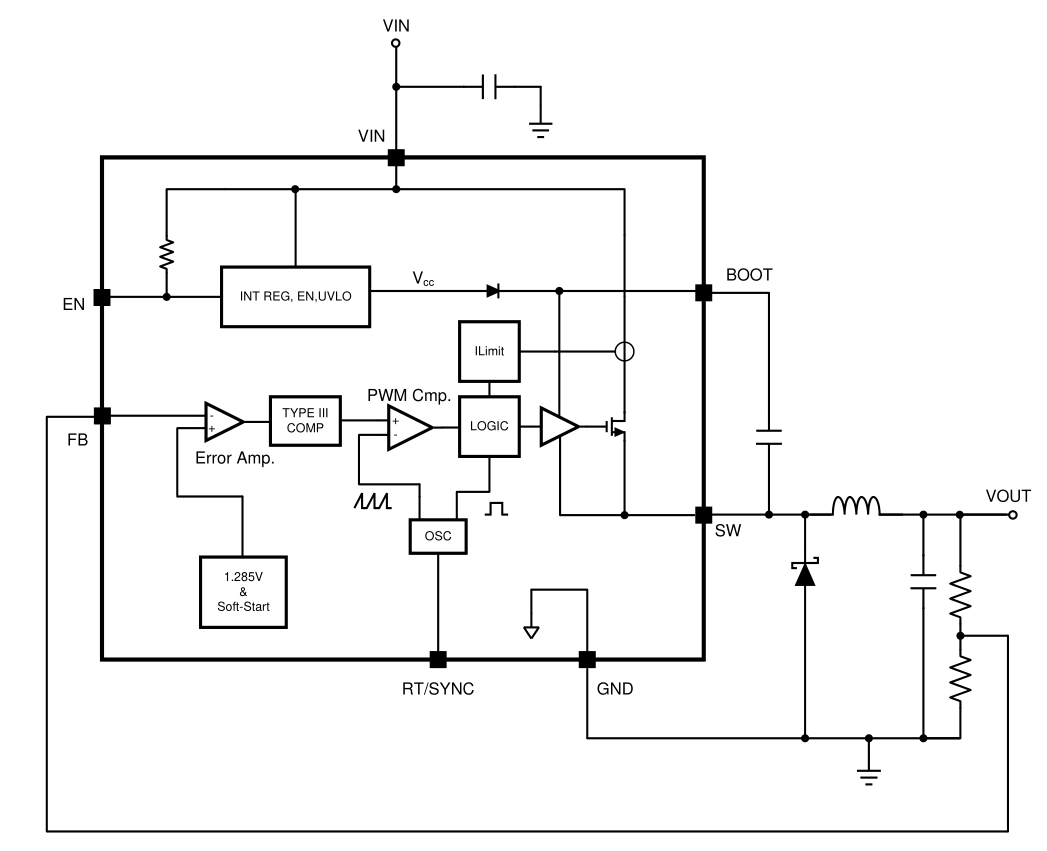
\includegraphics[scale=0.5]{../images/analog-lm22673-bloques}
    \caption{Diagrama de bloques del integrado LM22673-TJ-ADJ}
    \label{fig:analog-lm22673-bloques}
  \end{figure}

  En la \autoref{fig:analog-fuente-12v} se puede observar el esquemático de la fuente de \SI{12}{V}.

  \begin{figure}[!htbp]
    \centering
    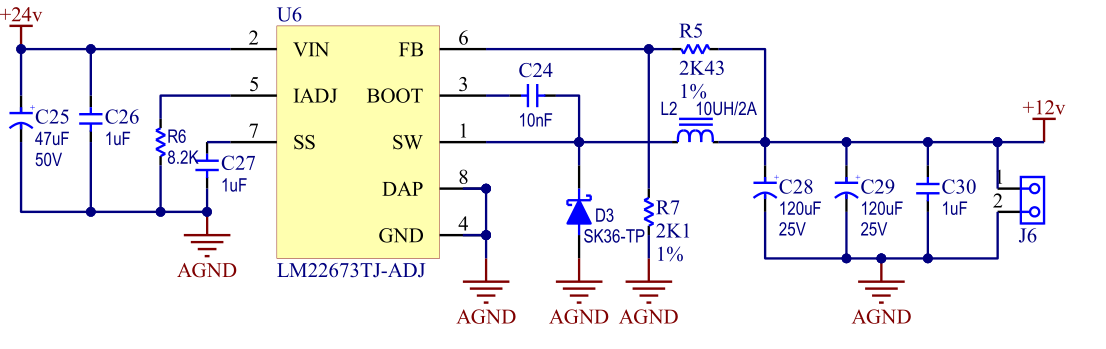
\includegraphics[scale=0.55]{../images/analog-fuente-12v}
    \caption{Fuente de alimentación de \SI{12}{V}}
    \label{fig:analog-fuente-12v}
  \end{figure}

  Siguiendo las indicaciones de la hoja de datos, se procedió a elegir los componentes:

  \begin{itemize}
    \item $C_2$ y $C_3$ conectados a $V_{IN}$. Esta combinación de capacitores de desacoplamiento, uno electrolítico grande y uno cerámico más pequeño, permite aislar al circuito de ruidos tanto de baja como de alta frecuencia provenientes de la fuente de tensión. También permite compensar las inductancias parásitas.
    \item $R_2$ conectado a $I_{ADJ}$. Este pin regula la corriente máxima pico. Una solo resistencia es necesaria entre este pin y masa para poder controlarla, de acuerdo a lo mostrado en la \autoref{fig:analog-lm22673-iadj}.

    \begin{figure}[!htbp]
      \centering
      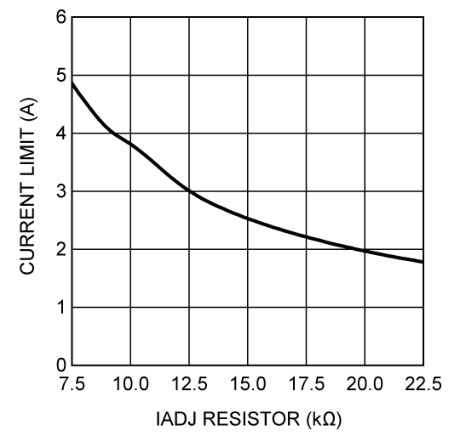
\includegraphics[scale=0.6]{../images/analog-lm22673-iadj.png}
      \caption{Corriente pico máxima vs. resistencia de $I_{ADJ}$ en LM22673-TJ-ADJ}
      \label{fig:analog-lm22673-iadj}
    \end{figure}

    \item $R_1$ y $R_3$ conectados a $FB$. Este pin permite ajustar la tensión generada, a partir de la correcta elección de valores de las resistencias. Se siguió la siguiente ecuación provista por el fabricante, siendo $R_{FBT}$ la resistencia entre $FB$ y $V_{OUT}$ y $R_{FBB}$ la resistencia entre $FB$ y masa.
      \[
        R_{FBT} = \left[ \frac{V_{out}}{1.285} - 1 \right] \cdot R_{FBB}
      \]

    \item $L_1$, $C_5$, $C_6$ y $C_7$ conectados a $SW$ formando así un filtro pasabajos para generar la tensión de salida.

    \item $C_1$ y $D_1$ conectados entre $BOOT$ y $SW$ y entre $SW$ y masa respectivamente. Este capacitor de bootstrapping genera en conjunto con el diodo la tensión necesaria para encender el MOSFET que se encuentra a la salida del integrado, tal como se observa en la \autoref{fig:analog-lm22673-bloques}. Se eligió además un diodo tipo Schottky, de acuerdo a las recomendaciones del fabricante, con una tensión reversa máxima  de 1.3 veces la máxima tensión de entrada.

    \item $C_4$ conectado a $SS$. Este pin permite regular la función \emph{soft-start} del integrado, reduciendo el tiempo que le toma llegar a estado estacionario y de esa forma someter a menor estrés al mismo. Fue elegido siguiendo la siguiente ecuación:
    \[
      T_{SS} \approx \num{26e3} \cdot C_{SS}
    \]
    tomando el máximo valor recomendado por el fabricante (de \SI{100}{nF} a \SI{1}{\micro F}), ya que no se necesitan mejores prestaciones.

  \end{itemize}

  %% ----------------------------------------------------------------
  \subsubsection{Fuente de alimentación de 5V y 1.8V}
  %% ----------------------------------------------------------------
  La fuente de \SI{5}{V} alimenta el conversor analógico digital, las fuentes de \SI{3.3}{V}, \SI{1.8}{V}, \SI{-5}{V} y los amplificadores operacionales empleados en la etapa de adquisición y adecuación de señales.

  La fuente de \SI{1.8}{V}, por otro lado, alimenta solamente el ADC.

  Dado el bajo costo y las relativamente bajas necesidades de potencia, se decidio utilizar una fuente lineal. Por motivos de disponibilidad se eligió el integrado LM1117 de tensión fija. El mismo tiene las siguientes características:

  \begin{itemize}
    \item Corriente máxima de \SI{800}{mA}
    \item Máxima regulación de carga del 0.4\%
    \item Mínima cantidad de componentes
  \end{itemize}

  El diagrama de bloques del integrado se puede ver en la \autoref{fig:analog-lm1117-bloques}

  \begin{figure}[!htbp]
    \centering
    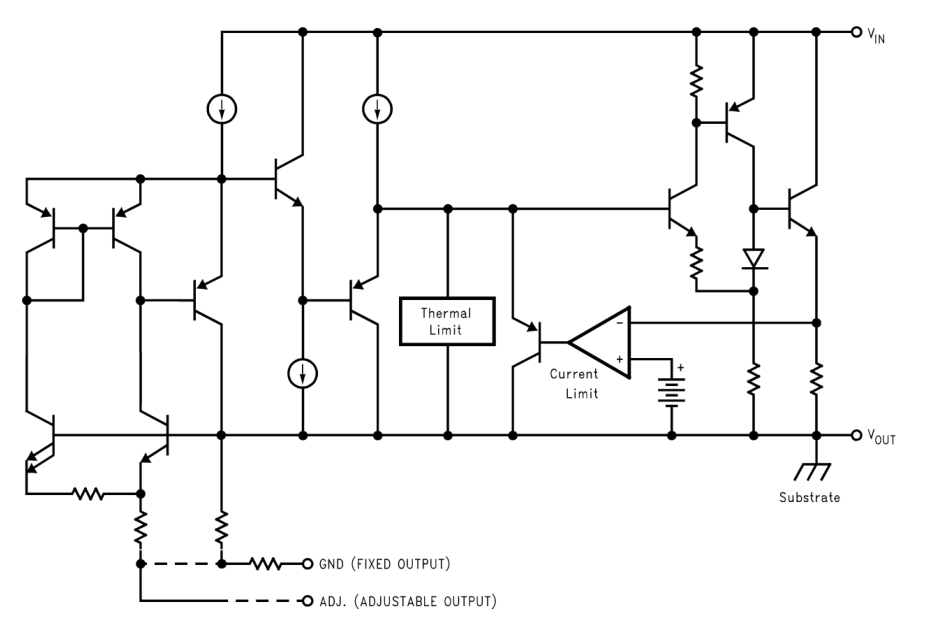
\includegraphics[scale=0.6]{../images/analog-lm1117-bloques.png}
    \caption{Diagrama de bloques del integrado LM1117MP-1.8/NOPB}
    \label{fig:analog-lm1117-bloques}
  \end{figure}

  En la \autoref{fig:analog-fuente-1v8} se puede observar el esquemático de la fuente de \SI{1.8}{V}. La versión utilizada del integrado es la LM1117MP-1.8.

  \begin{figure}[!htbp]
    \centering
    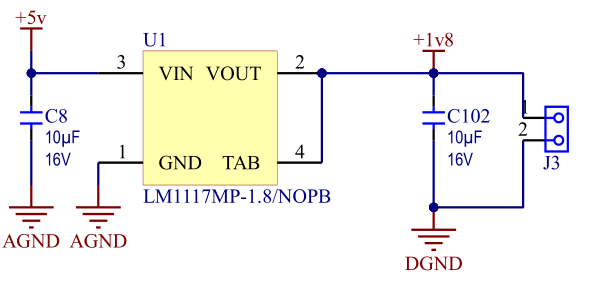
\includegraphics[scale=0.6]{../images/analog-fuente-1v8.png}
    \caption{Fuente de alimentación de \SI{1.8}{V}}
    \label{fig:analog-fuente-1v8}
  \end{figure}

  El esquemático de la fuente de \SI{5}{V} es idéntico, siendo en este caso el integrado LM1117MP-5.0, versión de tensión fija para \SI{5}{V}.

  %% ----------------------------------------------------------------
  \subsubsection{Fuente de alimentación de 3.3V}
  %% ----------------------------------------------------------------
  Esta fuente alimenta las siguientes partes del circuito: microcontrolador, ADC y driver del MOSFET. Dados los bajos requerimientos de potencia y el menor costo, se decidió utilizar una fuente lineal.

  De esta forma se eligió el integrado TPS79533DCQR. El mismo ha sido utilizado en diseños previos con un alto grado de confiabilidad. Entre sus características más destacables se encuentra:

  \begin{itemize}
    \item Corriente máxima de \SI{500}{mA}
    \item Muy bajo ruido (\SI{33}{\micro V_{RMS}})
    \item Baja caída de tensión a máxima carga (\SI{110}{mV})
    \item Mínima cantidad de componentes
  \end{itemize}

  El diagrama en bloques del integrado se puede ver en la \autoref{fig:analog-TPS79533DCQR-bloques}.

  \begin{figure}[!htbp]
    \centering
    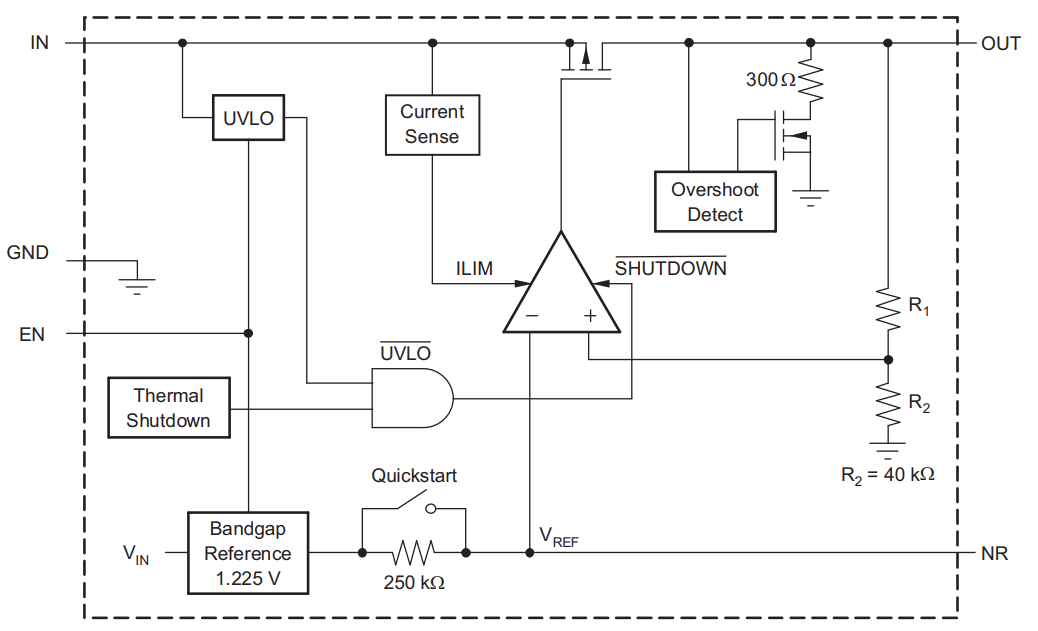
\includegraphics[scale=0.5]{../images/analog-TPS79533DCQR-bloques.png}
    \caption{Diagrama de bloques del integrado TPS79533DCQR}
    \label{fig:analog-TPS79533DCQR-bloques}
  \end{figure}

  En la \autoref{fig:analog-fuente-3v3} se puede observar el esquemático de la fuente de \SI{3.3}{V}.

  \begin{figure}[!htbp]
    \centering
    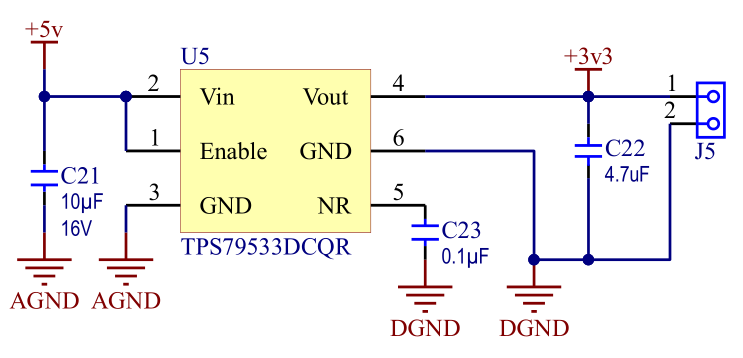
\includegraphics[scale=0.5]{../images/analog-fuente-3v3.png}
    \caption{Fuente de alimentación de \SI{3.3}{V}}
    \label{fig:analog-fuente-3v3}
  \end{figure}

  Siguiendo las indicaciones de la hoja de datos, se eligieron los componentes necesarios. Estos, tal como se puede observar, son simplemente tres capacitores, ya que este integrado permite un uso mínimo de componentes.

\end{document}